\subsubsection{Minimal Optimizations (\texttt{-O1})}

The \texttt{-O1} optimization level represents the first step beyond baseline execution, implementing several impacting changes as shown in Figure~\ref{fig:all_o1}.

\begin{figure}[H]
  \centering
  \noindent
  \makebox[0pt][c]{
    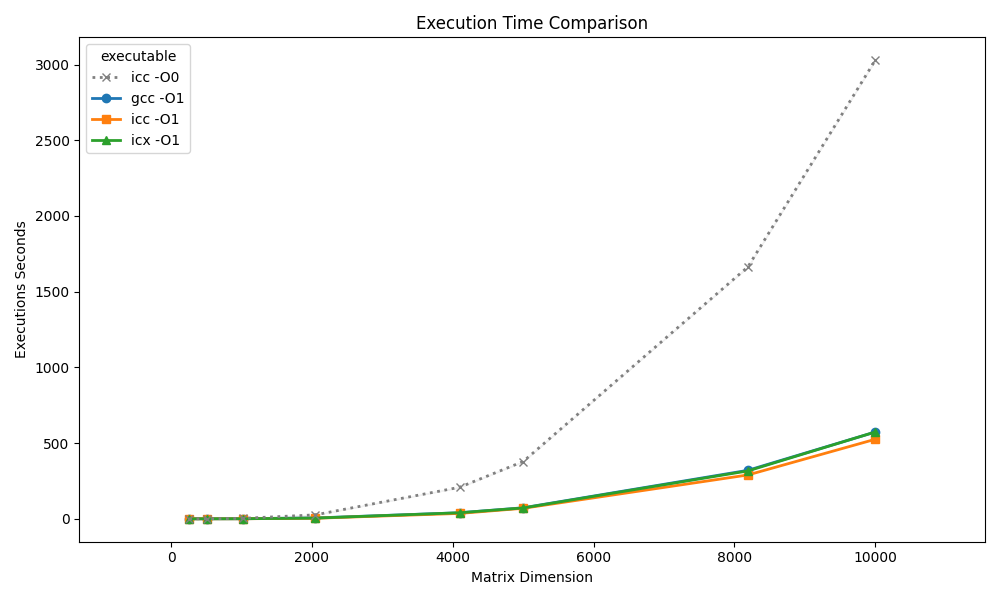
\includegraphics[width=0.6\paperwidth]{Images/all_o1.png}
  }
  \caption{Execution time scaling as a function of matrix size ($n$) at \texttt{-O1}.}
  \label{fig:all_o1}
\end{figure}

At this stage, the compiler enables basic scalar optimizations such as constant folding, dead code elimination, and limited inlining. However, aggressive loop transformations, cache blocking, and automatic vectorization remain inactive. 

The compiler optimization report confirms this behavior, repeatedly issuing the remark: 

\begin{quote}
    \texttt{remark \#15320: routine skipped: loop optimizations disabled}
\end{quote}

This indicates that loop-level optimizations and vectorization passes are not applied under the \texttt{-O1} profile. Consequently, the triple-nested loop is executed in scalar form, failing to exploit the AVX2 SIMD units available on the target architecture. 

Furthermore, the absence of loop restructuring prevents the compiler from improving data locality, leaving the implementation unable to effectively utilize the hardware's caching capabilities.

\paragraph{Intel Advisor Analysis.} 
The Intel Advisor Roofline analysis (Figure~\ref{fig:roofline_o1}) places the kernel in a strictly memory-bound regime. 

\begin{figure}[H]
    \centering
    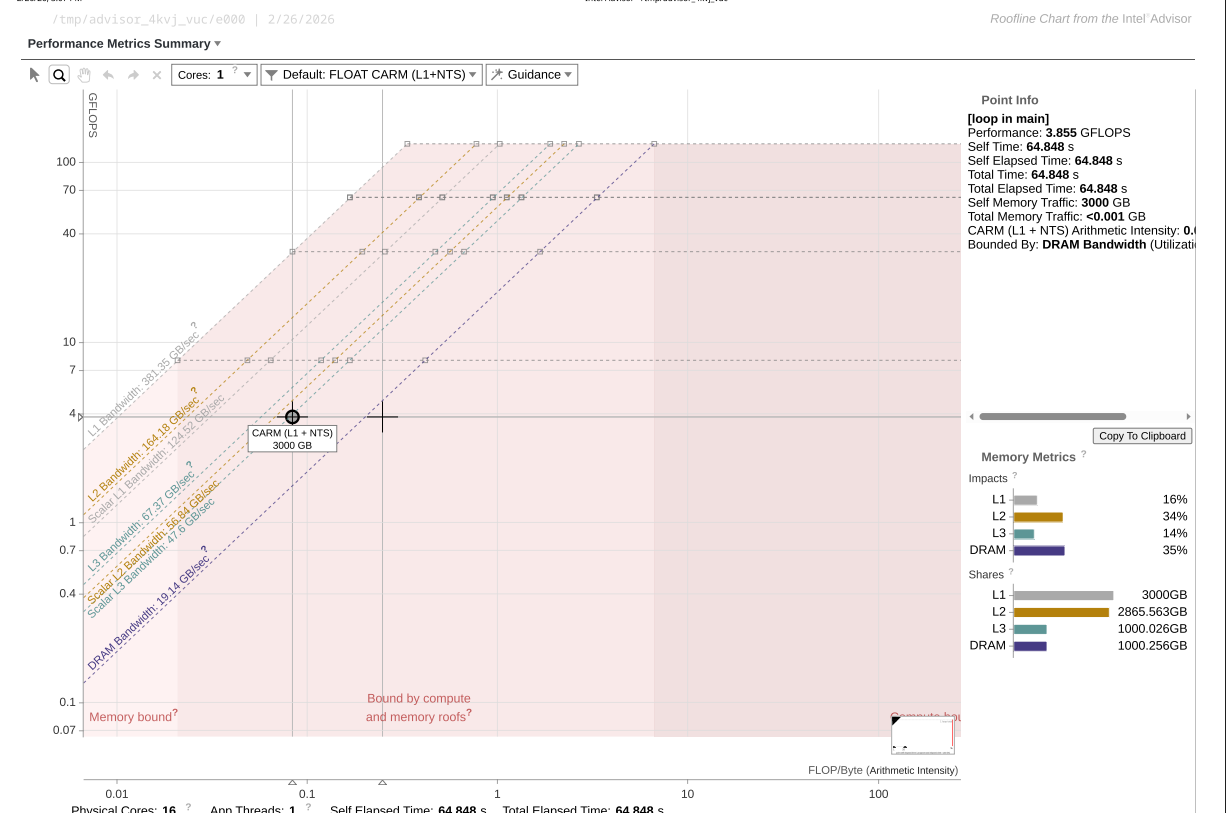
\includegraphics[width=1\textwidth]{Images/icc_o1_roofline.png}
    \caption{Intel Advisor Roofline analysis for ICC \texttt{-O1}.}
    \label{fig:roofline_o1}
\end{figure}

Measured performance reaches \textbf{3.855 GFLOPS}, with an arithmetic intensity of approximately 0.1 FLOP/Byte. Such low intensity indicates that the algorithm performs very few floating-point operations per byte transferred from memory. Execution is thus constrained by memory bandwidth rather than computational throughput, preventing the functional units from reaching their theoretical peak.

The memory hierarchy breakdown further clarifies these performance limitations:

\begin{itemize}
    \item \textbf{Stall Impact:} The dominant stall sources are DRAM (35\%) and L2 (34\%), accounting for nearly 70\% of total execution stalls. This confirms that latency at lower cache levels and main memory significantly limits pipeline utilization.
    \item \textbf{Traffic Distribution:} Memory traffic analysis reports approximately \textbf{3000 GB} of data passing through L1, with the majority propagating to L2 (2865 GB), and nearly 1000 GB reaching L3 and DRAM. This indicates insufficient temporal locality and poor cache residency of the working set.
\end{itemize}

\paragraph{valgrind insight}
Dynamic analysis via Valgrind further corroborates the memory-bound diagnosis. The key metrics for this configuration are summarized in Table~\ref{tab:cachegrind_results_o1}.

\begin{table}[H]
\centering
\caption{Key Valgrind Cachegrind memory profiling metrics for ICC \texttt{-O1} ($n=5000$).}
\label{tab:cachegrind_results_o1}
\begin{tabular}{lr}
\toprule
\textbf{Metric} & \textbf{Total Count / Rate} \\
\midrule
Instruction References (I) & 875,303,318,749 \\
Data References (D)        & 375,101,183,650 \\
\midrule
L1 Data Misses             & 31,309,389,456 \\
L1 Data Miss Rate          & 8.3\% (\textbf{12.5\% Read}) \\
\midrule
Last-Level (LL) Misses     & \textbf{15,640,645,313} \\
Last-Level (LL) Miss Rate  & 1.3\% (6.3\% Read) \\
\bottomrule
\end{tabular}
\end{table}


The L1 data cache exhibits a 12.5\% read miss rate, which is unusually high for high-performance workloads and indicates limited spatial locality within the innermost loop. 
The last-level cache (L3) shows a 6.3\% read miss rate, translating into approximately 15.6 billion accesses to main memory.

Although the overall LL miss rate (1.3\%) appears moderate, the extremely large number of total memory references amplifies the impact of each miss, resulting in substantial DRAM traffic and high latency penalties.

These findings are consistent with the Roofline model and confirm that memory latency and bandwidth represent the primary bottleneck under minimal optimization settings.

\paragraph{Conclusions. }
In summary, the \texttt{-O1} configuration introduces basic scalar optimizations but does not alter the algorithm's fundamental memory access pattern: the combined evidence identifies the kernel as \textbf{bandwidth-bound}.

The triple nested loop remains non-vectorized and untiled, leading to low arithmetic intensity and excessive off-chip memory traffic.

